%MB9T5
\setcounter{paragraph}{0}
\setcounter{ex}{0}
\PhanI
\loai{Điều kiện sóng dừng - Tìm bước sóng}
\begin{ex}%[3P2K8-2][Loai1]
Hai sóng dạng sin cùng bước sóng, cùng biên độ truyền ngược chiều nhau trên một sợi dây đàn với tốc độ 10 cm/s tạo ra một sóng dừng. Biết khoảng thời gian giữa hai thời điểm gần nhau nhất mà dây duỗi thẳng là 0,5 s. Bước sóng là
\choice
{5 cm}
{\True 10 cm}
{20 cm}
{25 cm}
\loigiai{
\begin{itemize}
\item Khoảng thời gian giữa hai lần liên tiếp sợi dây duỗi thẳng là $\dfrac{T}{2}=0,5\ s \Rightarrow T=1$ s.
\item Bước sóng: $\lambda = \dfrac{v}{f} = v.T = 10\ cm $.
\end{itemize}
}
\end{ex} \haidong{20}
\begin{ex}%[3P2K8-2][Loai1]
Một sợi dây dài $\ell=2$ m, hai đầu cố định. Người ta kích thích để có sóng dừng xuất hiện trên dây. Bước sóng dài nhất bằng
\choice
{1 m}
{2 m}
{\True 4 m}
{Không đủ điều kiện để xác định được}
\loigiai{
\begin{itemize}
\item Ta có: $\ell = \dfrac{k\lambda}{2}\Rightarrow \lambda = \dfrac{2\ell}{k} $.
\item Bước sóng dài nhất khi $k = 1 \Rightarrow \lambda = \dfrac{2.2}{1} = 4\ m$.
\end{itemize}
}
\end{ex} \haidong{20}

\begin{ex}%[3P2K8-2][Loai1]
Một sợi dây AB treo lơ lửng, đầu A gắn vào một nhánh của âm thoa có tần số f. Sóng dừng trên dây, người ta thấy khoảng cách từ B đến nút thứ 3 (kể từ B) là 5 cm. Bước sóng có giá trị là
\choice
{\True 4 cm}
{5 cm}
{8 cm}
{10 cm}
\loigiai{
\begin{itemize}
\item B là một bụng sóng. Gọi nút thứ 3 tính từ B là M thì $MB = \left( 2. 2+1 \right). \dfrac{\lambda }{4}\Rightarrow\lambda = 4$ cm.
\end{itemize}
}
\end{ex} \haidong{20}
\loai{Chiều dài dây}
\begin{ex}%[3P2B8-2][Loai1]
Một sợi dây AB căng ngang, đầu B cố định, đầu A gắn với một nhánh của âm thoa dao động điều hòa với tần số 25 Hz. Trên dây AB có một sóng dừng ổn định, A được coi là nút sóng. Tốc độ truyền sóng trên dây là 1,2 m/s. Tổng số bụng sóng và nút sóng trên dây là 27. Chiều dài của dây bằng
\choice
{0,312 cm}
{3,12 m}
{\True 31,2 cm}
{0,336 m}
\loigiai{
\begin{itemize}
\item Tổng số bụng và nút bằng 27 $\Rightarrow$ Số bụng $k = 13$ và số nút là 14 $\Rightarrow f=13. \dfrac{v}{2\ell}\Rightarrow \ell=31,2\ cm$.
\end{itemize}
}
\end{ex} \haidong{20}
\loai{Hai đầu cố định - Tìm số nút}
\begin{ex}%[3P2K8-2][Loai1]
Dây AB dài 30 cm căng ngang, hai đầu cố định, khi có sóng dừng thì tại N cách B khoảng 9 cm là nút thứ 3 (đếm từ đầu B và không kể B). Số nút trên dây AB (tính cả A và B) là
\choice
{9}
{10}
{\True 11}
{12}
\loigiai{
\begin{itemize}
\item M là nút thứ 3 kể từ B (không tính B) $\Rightarrow MB = 3. \dfrac{\lambda }{2}\Rightarrow \lambda = 6$ cm.
\item Số bụng sóng là: $k=\dfrac{\ell }{0,5\lambda }=10 \Rightarrow$ số nút là 11.
\end{itemize}
}
\end{ex} \haidong{20}
\loai{Hai đầu cố định - Tìm số bụng}
\begin{ex}%[3P2B8-2][Loai1]
Trên một sợi dây đàn hồi dài 1,2 m, hai đầu cố định, đang có sóng dừng. Biết sóng truyền trên dây có tần số 100 Hz và tốc độ 80 m/s. Số bụng sóng trên dây là
\choice
{\True 3}
{4}
{2}
{5}
\loigiai{
\begin{itemize}
\item Điều kiện xảy ra sóng dừng trên sợi dây: $\ell =k.\dfrac{\lambda }{2}=k.\dfrac{v}{2f}\Rightarrow k=\dfrac{2\ell f}{v}=\dfrac{2.1,2.100}{80}=3$.
\item Số bụng sóng trên sợi dây: $N_b=k=3$ bụng.
\end{itemize}}
\end{ex} \haidong{20}
\begin{ex}%[3P2K8-2][Loai1]
Một dây AB dài 90 cm có hai đầu A, B cố định. Dây được kích thích để trên dây có sóng dừng với khoảng cách giữa vị trí cân bằng của hai bụng ở xa nhất cách nhau 75 cm. Số bụng sóng trên dây là
\choice
{4}
{12}
{10}
{\True 6}
\loigiai{
\begin{itemize}
\item Ta có: $\Delta x=90-75=\dfrac{\lambda }{2}\Rightarrow \lambda =30$ cm.
\item Điều kiện để có sóng dừng trên dây với hai đầu cố định: $\ell=k\dfrac{\lambda }{2}\Rightarrow k=6\Rightarrow $ trên dây có 6 bụng sóng.
\end{itemize}
}
\end{ex} \haidong{20}
\begin{ex}%[3P2K8-2][Loai1]
Dây AB dài 40 cm căng ngang, hai đầu cố định, khi có sóng dừng thì tại M là bụng thứ 4 (kể từ B), biết $BM = 14$ cm. Số bụng sóng trên dây AB là
\choice
{9}
{\True 10}
{11}
{12}
\loigiai{
\begin{itemize}
\item M là bụng thứ 4 kể từ B $\Rightarrow MB = \left(2.4-1 \right).\dfrac{\lambda }{4} \Rightarrow \lambda = 8$ cm.
\item Số bụng sóng là: $n=\dfrac{\ell }{0,5\lambda }=10$.
\end{itemize}
}
\end{ex} \haidong{20}
\loai{Hai đầu cố định. Cho số nút. Tìm tốc độ truyền sóng}
\begin{ex}%[3P2B8-2][Loai1]
Trên một sợi dây đàn hồi dài 80 cm với hai đầu A và B cố định đang có sóng dừng, tần số sóng là 50 Hz. Không kể hai đầu A và B, trên dây có 7 nút sóng. Tốc độ truyền sóng trên dây là
\choice
{20 m/s}
{15 m/s}
{25 m/s}
{\True 10 m/s}
\loigiai{
\begin{itemize}
\item Ta có: $8\dfrac{\lambda}{2} = 80 \Rightarrow \lambda = 20\ cm \Rightarrow v = \lambda.f = 20.50 = 1000\ cm /s = 10\ m/s$.
\end{itemize}
}\end{ex} \haidong{20}
\begin{ex}%[3P2K8-2][Loai1]
Trong thí nghiệm về sóng dừng, trên một sợi dây đàn hồi dài 1,2 m với hai đầu cố định, người ta quan sát thấy ngoài hai đầu dây cố định còn có hai điểm khác trên dây không dao động. Biết khoảng thời gian giữa hai lần liên tiếp với sợi dây duỗi thẳng là 0,05 s. Tốc độ truyền sóng trên dây là
\choice
{\True 8 m/s}
{4 m/s}
{12 m/s}
{16 m/s}
\loigiai{
\begin{itemize}
\item Dây có 4 nút tất cả $\Rightarrow$ có 3 bụng.
\item $T = 0,1\ s \Rightarrow f = 10\ Hz = 3. \dfrac{v}{2\ell } \Rightarrow v = 8\ m/s$.
\end{itemize}
}
\end{ex} \haidong{20}

\loai{Hai đầu cố định. Cho số bụng. Tìm tốc độ truyền sóng}
\begin{ex}%[3P2B8-2][Loai1]
Trên một sợi dây đàn hồi dài 1,8 m, hai đầu cố định, đang có sóng dừng với 6 bụng sóng. Biết sóng truyền trên dây có tần số 100 Hz. Tốc độ truyền sóng trên dây là
\choice
{50 m/s}
{70 m/s}
{\True 60 m/s}
{80 m/s}
\loigiai{
\begin{itemize}
\item Số bụng sóng: $N_b=k=6$.
\item Điều kiện để có sóng dừng trên sợi dây hai đầu cố định:
\begin{align*}
\ell =k.\dfrac{\lambda}{2}=k.\dfrac{v}{2f}\Rightarrow v=\dfrac{2f\ell}{k}=\dfrac{2.100.1,8}{6}=60\ \ m/s.
\end{align*}
\end{itemize}
}\end{ex} \haidong{20}
\begin{ex}%[3P2K8-2][Loai1]
Một sợi dây đàn hồi có độ dài $AB=80$ cm, đầu B giữ cố định, đầu A gắn cần rung dao động điều hoà với tần số 50 Hz theo phương vuông góc với AB. Trên dây có một sóng dừng với 4 bụng sóng, coi A, B là hai nút sóng. Tốc độ truyền sóng trên dây là
\choice
{\True 20 m/s}
{30 m/s}
{5 m/s}
{40 m/s}
\loigiai{
\begin{itemize}
\item Sóng dừng với hai đầu cố định với 4 bụng sóng khi đó ta có $\Rightarrow \ell = \dfrac{4\lambda }{2} \Rightarrow v=20\ m/s$.
\end{itemize}
}
\end{ex} \haidong{20}
\loai{Hai đầu cố định. Tự xác định số nút, bụng. Tìm tốc độ truyền sóng}
\begin{ex}%KNTT
Một lò xo có chiều dài 1,2 m, đầu trên gắn vào một nhánh âm thoa, đầu dưới treo một quả cân. Dao động của âm thoa được duy trì bằng một nam châm điện để có tần số 50 Hz. Khi đó, trên lò xo có sóng dừng và trên lò xo chỉ có một nhóm vòng dao động với biên độ cực đại. Tốc độ truyền sóng trên lò xo là
\choice
{\True 120 m/s}
{130 m/s}
{140 m/s}
{150 m/s}
\loigiai{
\begin{itemize}
\item Trên lò xo chỉ có một bụng nên: $\ell=\dfrac{\lambda}{2}\Rightarrow \lambda=2\ell=2,4\ m$. 
\item Do đó: $v=\lambda f=120\ m/s$.
\end{itemize}
}
\end{ex} \haidong{20}

\begin{ex}%KNTT
\immini[thm]{
Trên sợi dây đàn hồi, có chiều dài $L=1,2\ m$ người ta tạo ra sóng dừng có hình dạng được mô tả ở hình bên. Biết tần số rung của sợi dây là $f=13,3\ Hz$. Tốc độ truyền sóng trên dây là
\motcot
{\True 10,64 m/s}
{5,64 m/s}
{15,45 m/s}
{4,54 m/s}
}{\begin{tikzpicture}[draw=Mapcolor,scale=0.7,thick,>=stealth',rotate=-90]
\draw[very thick] (0,-0.5)--(0,0.5)(4.5,-0.5)--(4.5,0.5);
\draw [Mapcolor,line width = 1.2pt, domain=0:4.5, samples=500]%
plot (\x, {0.5*cos(\x*120-90)});
\draw [Mapcolor,line width = 1.2pt, domain=0:4.5, samples=500]%
plot (\x, {0.5*cos(\x*120+90)});
\draw[<->](0,-0.75)--node[midway,left]{$L$}(4.5,-0.75);
\end{tikzpicture}}
\loigiai{
\begin{itemize}
\item Bước sóng: $\lambda=\dfrac{1,2}{1,5}=0,8\ m.$ 
\item Tốc độ truyền sóng: $v=\lambda.f=10,64\ m/s$. 
\end{itemize}
}
\end{ex} \haidong{20}

\loai{Một đầu cố định. Cho số bụng. Tìm tốc độ truyền sóng}
\begin{ex}%[3P2B8-2][Loai1]
Trên một sợi dây đàn hồi căng ngang có sóng dừng, M là một bụng sóng còn N là một nút sóng. Biết trong khoảng MN có 3 bụng sóng khác, $MN=63$ cm, tần số của sóng $f=20$ Hz. Bước sóng và vận tốc truyền sóng trên dây là
\choice
{$\lambda =3,6$ cm; $v=7,2$ m/s}
{$\lambda =3,6$ cm; $v=72$ cm/s}
{$\lambda =36$ cm; $v=72$ cm/s}
{\True $\lambda =36$ cm; $v=7,2$ m/s}
\loigiai{
\begin{itemize}
\item Ta có: $3,5 \dfrac{\lambda}{2} = MN \Rightarrow \lambda = \dfrac{2.MN}{3,5} = \dfrac{2.63}{3,5} = 36\ cm\Rightarrow v = \lambda.f = 36.20 = 720\ cm /s = 7,2\ m/s$.
\end{itemize}
}
\end{ex} \haidong{20}
\loai{Thay đổi chiều dài dây}
\begin{ex}%[3P2K8-2][Loai1]
Trên thanh AB đàn hồi với hai đầu cố định đang có một sóng dừng với tần số bằng 45 Hz. Buông đầu B cho tự do thì để trên thanh vẫn có sóng dừng cần phải rút ngắn độ dài thanh đi một đoạn nhỏ nhất bằng 6 cm. Tốc độ truyền sóng trên thanh bằng
\choice
{5 m/s}
{\True 10,8 m/s}
{15 m/s}
{20 m/s}
\loigiai{
\begin{itemize}
\item Khi hai đầu dây cố định thì $\ell = k\dfrac{\lambda}{2}$.
\item Sau khi để đầu B tự do, để thanh vẫn có sóng dừng thì cần rút ngắn đi một lượng nhỏ nhất 
\begin{align*}
\Delta \ell_{\min} = \dfrac{\lambda}{4} = 6 \Rightarrow \lambda = 24\ cm \Rightarrow v = \lambda.f = 24.45 = 1080\ cm /s = 10,8\ m/s.
\end{align*}
\end{itemize}
}
\end{ex} \haidong{20}
\loai{Điều kiện kẹp - Tìm bước sóng}
\begin{ex}%[3P2K8-2][Loai1]
Một sợi dây có chiều dài 1,5 m một đầu cố định một đầu tự do. Kích thích cho sợi dây dao động với tần số 100 Hz thì trên dây xuất hiện sóng dừng. Tốc độ truyền sóng trên dây nằm trong khoảng từ 150 m/s đến 400 m/s. Xác định bước sóng.
\choice
{14 m}
{\True 2 m}
{6 m}
{1 cm}
\loigiai{
\begin{itemize}
\item Ta có: $\ell=\left(2k-1\right)\dfrac{\lambda}{4}=\left(2k-1\right)\dfrac{v}{4f}\Rightarrow v=\dfrac{4\ell f}{\left(2k-1\right)}=\dfrac{600}{2k-1}$.
\item Theo đề: $150\le \dfrac{600}{2k-1}\le 400\Rightarrow 1,25\le k\le 2,5\Rightarrow k=2\Rightarrow v=200\ m/s\Rightarrow \lambda =\dfrac{v}{f}=2\ m$.
\end{itemize}
}
\end{ex} \haidong{20}
\begin{ex}%CTST
\immini[thm]{
Hiện tượng sóng dừng có thể xảy ra đối với sóng điện từ và có nhiều ứng dụng trong cuộc sống. Ví dụ trong lò vi sóng (lò vi ba), sóng điện từ được phản xạ trên các thành lò và tạo thành sóng dừng trong lò. Tại những bụng sóng, năng lượng của sóng điện từ có giá trị lớn nhất và cung cấp nhiệt cho thực phẩm (từ sự dao động của các phân tử nước trong thực phẩm). Do đó, trong lò vi ba còn có đĩa quay để giúp thực phẩm nóng đều}{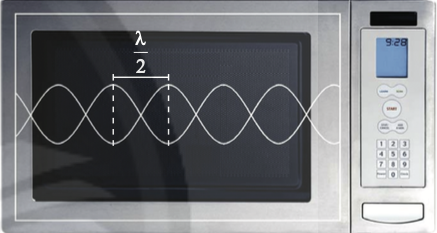
\includegraphics[width=4cm]{Hinh/CT913}}
Trong một thử nghiệm nướng bánh bằng lò vi sóng, người ta đo được khoảng cách giữa hai phần nóng nhất và gần nhau nhất của bánh là khoảng 6,13 cm. Biết tần số sóng vi ba được sử dụng trong lò là 2,45 GHz. Sử dụng các số liệu đã cho để ước lượng tốc độ lan truyền của sóng điện từ là bao nhiêu?
\choice
{\True $3.10^8\ m/s$}
{$3.10^7\ m/s$}
{$2,9.10^8\ m/s$}
{$3,2.10^8\ m/s$}
\loigiai{
\begin{itemize}
\item $\lambda=2.6,13=12,26\ cm$.
\item $v=\lambda.f=0,1226.2,45.10^9\approx 3.10^8\ m/s$.
\end{itemize}
}
\end{ex} \haidong{20}
\setcounter{paragraph}{0}
\setcounter{ex}{0}
\PhanII
\begin{ex}
Hình vẽ dưới đây mô tả sóng dừng trên một sợi dây có chiều dài $L=0,9 \  m$, hai đầu cố định.\\
\centerline{\begin{tikzpicture}[draw=Mapcolor,very thick,>=stealth']
\pgfplotsset{width=8cm,height=3.5cm,compat=1.4}
\begin{axis}[
axis lines=none,
xmin=0,xmax=6.5,xstep=1,ymin=-1.6,ymax=3.5,ystep=1,
grid=none, %Có các tùy chọn: minor|major|both|none
x grid style={dashed},
y grid style={dashed},
ytick={-1.5,-1,-0.5,0,0.5,1,1.5},
xtick={0.33,0.66,...,6},
xticklabels={},
yticklabels={},
xticklabel style={below},
xlabel style={above=1 pt},
xlabel=$x(cm)$,
ylabel style={left=2pt},
ylabel={$u$}
]
\addplot[line width=1.2pt,domain=0:6,samples=200,Mapcolor]{1.5*cos(deg(0.5*pi*x-pi/2))};
\addplot[line width=1.2pt,domain=0:6,samples=200,Mapcolor]{1.5*cos(deg(0.5*pi*x+pi/2))};
\draw[<->,very thick] (axis cs: 0, 2)--node[midway,above]{L}(axis cs: 6, 2);
\end{axis}
\end{tikzpicture}}
\choiceTF[t]
{\True Trên dây có 3 bụng sóng và 4 nút sóng}
{\True Bước sóng $\lambda$ của sóng trên dây là 60 cm}
{\True Biết tần số là 180 Hz , tốc độ của sóng là $108 \  m/s$}
{Thay đổi tần số đến 360 Hz thì bước sóng bây giờ là $1,2 \  m$}
\loigiai{
\begin{itemchoice}
\itemch Từ hình vẽ có 3 bụng sóng, hai đầu cố định là 2 nút, vậy có 4 nút sóng. Đúng.
\itemch $L = n \dfrac{\lambda}{2} \Rightarrow 0.9 = 3 \dfrac{\lambda}{2} \Rightarrow \lambda = 0.6 \  m = 60 \  cm$. Đúng.
\itemch $v = \lambda f = 0.6 . 180 = 108 \  m/s$. Đúng.
\itemch $v$ không đổi, $\lambda' = v/f' = 108/360 = 0.3 \  m = 30 \  cm$. Đúng.
\end{itemchoice}
}
\end{ex}
\begin{ex}
Một sợi dây AB có đầu B được gắn chặt và đầu A gắn vào một âm thoa có tần số dao động $f$. Cho âm thoa dao động ta quan sát thấy trên dây có sóng dừng với hai đầu $A$, $B$ đều là nút sóng. Tại $M$ là bụng thứ 3 tính từ $B$, với $MB=10\ cm$. Biết $AB=20\ cm$, $f=10\ Hz$.
\choiceTF[t]
{\True Trên dây xuất hiện 6 nút sóng và 5 bụng sóng}
{\True Tốc độ truyền sóng trên dây là $80\ cm/s$}
{Khoảng cách giữa 3 nút sóng liên tiếp là $12\ cm$}
{Khoảng cách giữa 4 bụng liên tiếp là $8\ cm$}
\loigiai{
\begin{itemchoice}
\itemch Vì hai đầu A và B là nút sóng, chiều dài sợi dây $l = k \dfrac{\lambda}{2}$, với $k$ là số bụng sóng. M là bụng thứ 3 tính từ B, nên $MB = (3 - \dfrac{1}{2}) \dfrac{\lambda}{2} = \dfrac{5\lambda}{4} = 10 cm \Rightarrow \lambda = 8\ cm$. Chiều dài dây $AB = 20 cm = k \dfrac{8 cm}{2} \Rightarrow k = 5$. Vậy trên dây có 5 bụng sóng và $5 + 1 = 6$ nút sóng (kể cả hai đầu).
\itemch Tốc độ truyền sóng trên dây là $v = f \lambda = 10 Hz . 8 cm = 80 cm/s$.
\itemch Khoảng cách giữa hai nút sóng liên tiếp là $\dfrac{\lambda}{2} = \dfrac{8 cm}{2} = 4\ cm$. Vậy khoảng cách giữa 3 nút sóng liên tiếp là $2 . 4 cm = 8\ cm$.
\itemch Khoảng cách giữa hai bụng sóng liên tiếp là $\dfrac{\lambda}{2} = \dfrac{8 cm}{2} = 4\ cm$. Vậy khoảng cách giữa 4 bụng sóng liên tiếp là $3 . 4 cm = 12\ cm$.
\end{itemchoice}
}
\end{ex}
\begin{ex}
Một sợi dây AB dài $22\ cm$ với đầu A gắn vào cần rung tạo sóng, đầu B cố định. Trên dây có sóng dừng với tần số $50\ Hz$, tốc độ truyền sóng trên dây là $4\ m/s$.
\choiceTF[t]
{\True Chiều dài $\ell$ của sợi dây thỏa mãn biểu thức $\ell=n . \dfrac{\lambda}{2}$ với $n=1,\ 2,\ 3, \dots$}
{Thời gian giữa 2 lần dây duỗi thẳng là $0,02\ s$}
{Khoảng cách giữa 4 nút sóng liên tiếp là $10\ cm$}
{\True Khoảng cách giữa 3 bụng liên tiếp là $8\ cm$}
\loigiai{
\begin{itemchoice}
\itemch Với một sợi dây có một đầu cố định và một đầu dao động tạo nút sóng (coi như cố định), điều kiện để có sóng dừng là chiều dài dây bằng một số nguyên lần nửa bước sóng: $l = n \dfrac{\lambda}{2}$, với $n$ là số bụng sóng.
\itemch Tần số sóng là $f = 50 Hz$, vậy chu kì sóng là $T = \dfrac{1}{f} = \dfrac{1}{50} s = 0,02 s$. Thời gian giữa hai lần dây duỗi thẳng liên tiếp là nửa chu kì, $\dfrac{T}{2} = \dfrac{0,02 s}{2} = 0,01 s$.
\itemch Bước sóng $\lambda = \dfrac{v}{f} = \dfrac{4 m/s}{50 Hz} = 0,08 m = 8\ cm$. Khoảng cách giữa hai nút sóng liên tiếp là $\dfrac{\lambda}{2} = \dfrac{8 cm}{2} = 4\ cm$. Vậy khoảng cách giữa 4 nút sóng liên tiếp là $3 . 4 cm = 12\ cm$.
\itemch Khoảng cách giữa hai bụng sóng liên tiếp là $\dfrac{\lambda}{2} = \dfrac{8 cm}{2} = 4\ cm$. Vậy khoảng cách giữa 3 bụng liên tiếp là $2 . 4 cm = 8\ cm$.
\end{itemchoice}
}
\end{ex}















\begin{ex}
Trên một sợi dây đàn hồi với hai đầu cố định đang có sóng dừng với bước sóng $2 \ cm$.\\
\choiceTF[t]
{\True Chiều dài sợi dây có thể nhận giá trị $9 \ cm$}
{Khoảng cách ngắn nhất giữa một nút và một bụng là $1 \ cm$}
{Giả sử sợi dây có chiều dài $\ell$. Trên dây đang có sóng dừng với $n$ bụng sóng, tốc độ truyền sóng trên dây là v. Khoảng thời gian giữa hai lần liên tiếp sợi dây duỗi thẳng là $\dfrac{\ell}{2 nv}$}
{Khi sợi dây duỗi thẳng thì tỉ số giữa chiều dài sợi dây và bước sóng bằng $n+0,5$ $(n=1;\ 2;\ 3;\ \ldots)$}
\loigiai{
\begin{itemchoice}
\itemch Vì $\ell=k \dfrac{\lambda}{2}=k \dfrac{2}{2}=k\ cm, k=1,2,3, \ldots$.
\itemch Vì khoảng cách ngắn nhất giữa một nút và một bụng là $\dfrac{\lambda}{4}=\dfrac{2}{4}=0,5 \ cm$
\itemch Vì khoảng thời gian liên tiếp hai lần dây duỗi thẳng là nửa chu kì. \\Ta có: $\ell=k \dfrac{\lambda}{2} \Rightarrow \ell=k \dfrac{vT}{2} \Rightarrow \dfrac{T}{2}=\dfrac{\ell}{kv}=\dfrac{\ell}{nv}$
\itemch Ta có: $\ell=k \dfrac{\lambda}{2} \Rightarrow \dfrac{\ell}{\lambda}=\dfrac{k}{2}=\dfrac{n}{2}=0,5 n$
\end{itemchoice}
}
\end{ex} \haidong{20}
\setcounter{paragraph}{0}
\setcounter{ex}{0}
\PhanIII
\begin{ex}
Một sợi dây đàn hồi dài $100 \ cm$ với hai đầu A và B cố định đang có sóng dừng, tần số sóng là $50 \ Hz$. Không kể hai đầu A và B, trên dây có 3 nút sóng. Tốc độ truyền sóng trên dây là bao nhiêu $m/s$?
\shortans[oly]{25}
\loigiai{
Ta có $: \ell=k \dfrac{\lambda}{2} \Rightarrow \ell=k \dfrac{v}{2 f} \Rightarrow v=\dfrac{2 f \ell}{k}=\dfrac{2.50.1}{4}=25 \ m/s$
}
\end{ex} \haidong{20}
\begin{ex}
Trên một sợi dây đang có sóng dừng ổn định. Khoảng cách ngắn nhất giữa một nút sóng và một bụng sóng liền kề là $3 \ cm$. Sóng truyền trên dây có bước sóng bằng bao nhiêu cm?
\shortans[oly]{12}
\loigiai{
$$
\dfrac{\lambda}{4}=3 \Rightarrow \lambda=12 \ cm
$$
}
\end{ex} \haidong{20}
\begin{ex}
Một sợi dây đàn hồi AB có hai đầu cố định và chiều dài $1,8 \ m$ đang lan truyền sóng dừng với tần số dao động $10 \ Hz$. Tốc độ truyền sóng trên sợi dây là $3 \ m/s$. Có bao nhiêu nút sóng trên dây?
\shortans[oly]{13}
\loigiai{
13
}
\end{ex} \haidong{20}
\begin{ex}
Một sợi dây AB có chiều dài $1 \ m$ căng ngang, đầu A cố định, đầu B gắn với một nhánh của âm thoa dao động điều hoà với tần số $20 \ Hz$. Trên dây có một sóng dừng ổn định với 4 bụng sóng, B được coi là nút sóng. Tốc độ truyền sóng trên dây là bao nhiêu $m/s$?
\shortans[oly]{10}
\loigiai{
10
}
\end{ex} \haidong{20}
\begin{ex}
Quan sát sóng dừng trên sợi dây AB, đầu A dao động điều hòa theo phương vuông góc với sợi dây (coi A là nút). Đầu B tự do và tần số dao động của đầu A là 20 Hz thì trên dây có sóng dừng ổn định với 6 nút sóng. Tốc độ truyền sóng trên dây là $20 \ m/s$. Chiều dài sợi dây bằng bao nhiêu mét (làm tròn kết quả đến chữ số hàng phần trăm)?
\shortans[oly]{2,75}
\loigiai{

}
\end{ex}
\begin{ex}
Một sợi dây đàn hồi dài 100 cm được nối một đầu với âm thoa (coi là một điểm cố định), đầu kia giữ cố định. Âm thoa dao động với tần số 20 Hz thì tạo ra sóng dừng trên dây. Cho biết tốc độ truyền sóng là $5 \ m/s$. Số bụng sóng trên dây có giá trị là bao nhiêu?
\shortans[oly]{8}
\loigiai{
Chiều dài sợi dây $L = 100$ cm = 1 m.
Tần số sóng $f = 20$ Hz.
Tốc độ truyền sóng $v = 5$ m/s.
Bước sóng $\lambda = v/f = 5/20 = 0,25$ m = 25 cm.
Với hai đầu cố định, điều kiện để có sóng dừng là $L = k \dfrac{\lambda}{2}$, với k là số bụng sóng.
$100 = k \dfrac{25}{2} \Rightarrow k = \dfrac{100 . 2}{25} = 8$.
Vậy trên dây có 8 bụng sóng.
}
\end{ex}